% Options for packages loaded elsewhere
\PassOptionsToPackage{unicode}{hyperref}
\PassOptionsToPackage{hyphens}{url}
\documentclass[
  11pt,
]{article}
\usepackage{xcolor}
\usepackage[margin=22mm]{geometry}
\usepackage{amsmath,amssymb}
\setcounter{secnumdepth}{-\maxdimen} % remove section numbering
\usepackage{iftex}
\ifPDFTeX
  \usepackage[T1]{fontenc}
  \usepackage[utf8]{inputenc}
  \usepackage{textcomp} % provide euro and other symbols
\else % if luatex or xetex
  \usepackage{unicode-math} % this also loads fontspec
  \defaultfontfeatures{Scale=MatchLowercase}
  \defaultfontfeatures[\rmfamily]{Ligatures=TeX,Scale=1}
\fi
\usepackage{lmodern}
\ifPDFTeX\else
  % xetex/luatex font selection
\fi
% Use upquote if available, for straight quotes in verbatim environments
\IfFileExists{upquote.sty}{\usepackage{upquote}}{}
\IfFileExists{microtype.sty}{% use microtype if available
  \usepackage[]{microtype}
  \UseMicrotypeSet[protrusion]{basicmath} % disable protrusion for tt fonts
}{}
\makeatletter
\@ifundefined{KOMAClassName}{% if non-KOMA class
  \IfFileExists{parskip.sty}{%
    \usepackage{parskip}
  }{% else
    \setlength{\parindent}{0pt}
    \setlength{\parskip}{6pt plus 2pt minus 1pt}}
}{% if KOMA class
  \KOMAoptions{parskip=half}}
\makeatother
\usepackage{graphicx}
\makeatletter
\newsavebox\pandoc@box
\newcommand*\pandocbounded[1]{% scales image to fit in text height/width
  \sbox\pandoc@box{#1}%
  \Gscale@div\@tempa{\textheight}{\dimexpr\ht\pandoc@box+\dp\pandoc@box\relax}%
  \Gscale@div\@tempb{\linewidth}{\wd\pandoc@box}%
  \ifdim\@tempb\p@<\@tempa\p@\let\@tempa\@tempb\fi% select the smaller of both
  \ifdim\@tempa\p@<\p@\scalebox{\@tempa}{\usebox\pandoc@box}%
  \else\usebox{\pandoc@box}%
  \fi%
}
% Set default figure placement to htbp
\def\fps@figure{htbp}
\makeatother
\setlength{\emergencystretch}{3em} % prevent overfull lines
\providecommand{\tightlist}{%
  \setlength{\itemsep}{0pt}\setlength{\parskip}{0pt}}
\usepackage{bookmark}
\IfFileExists{xurl.sty}{\usepackage{xurl}}{} % add URL line breaks if available
\urlstyle{same}
\hypersetup{
  hidelinks,
  pdfcreator={LaTeX via pandoc}}

\author{}
\date{}

\begin{document}

\section{Cauchy data from jumps and
residues}\label{cauchy-data-from-jumps-and-residues}

A boundary value contains several normal derivatives. They form a
weighted vector: taking another normal derivative costs one Sobolev
order. The central construction below acts on this entire vector. Its
leading symbol separates the modes entering the interior from the modes
entering the exterior; its full operator is a projection up to a smooth
kernel. Establishing that last assertion requires control of
distributions at the boundary, beyond a calculation of eigenvalues.

This lesson treats smooth elliptic differential operators of arbitrary
positive integer order on complex bundles of arbitrary common finite
rank. It neither assumes a scalar factorization nor prescribes the
number of boundary equations. The subsequent Fredholm theorem for
complementing boundary problems is a separate unit.

The analytic prerequisites are \href{stable-boundary-models.pdf}{Stable
modes and the algebra of boundary data}, Sections 1--3, for matrix ODE
modes; \href{conormal-transmission.pdf}{Singularities along a submanifold
and smooth boundary passage}, Sections 10--13, for ordinary transmission
and all layer traces; and
\href{geometric-microlocal-calculus.pdf}{Detecting regularity without
choosing coordinates}, Sections 5--6, 11 and 13, for properly supported
bundle operators, two-sided parametrices and Sobolev bounds. We also use
finite-dimensional linear algebra, smooth partitions of unity, Fourier
inversion, distributional differentiation, smooth local flows and
inverse functions, compactness, and the fundamental theorem of calculus.
The projection is constructed directly from these tools; the later
boundary Fredholm argument and all-real-order Poisson estimates are
separate.

\subsection{1. The weighted space of boundary
jets}\label{the-weighted-space-of-boundary-jets}

Let \(X\) be a compact smooth manifold with boundary \(Y\), let
\(E,F\to X\) be complex smooth bundles of common rank \(N\), and let \[
P:C^\infty(X;E)\longrightarrow C^\infty(X;F)
\tag{CD1}
\] be differential, elliptic, and of order \(m\geq1\). Ellipticity means
that its principal symbol \(p(x,\xi):E_x\to F_x\) is invertible for
every nonzero real covector. Sections here are ordinary bundle sections.
Choose a positive smooth density and Hermitian metrics for norms and
distributional duality; these choices do not change the operator
convention.

Fix an inward collar coordinate \(t\geq0\) and an identification of the
bundles in the collar with pullbacks from \(Y\), constructed in Section
4. Write \(D_t=-i\partial_t\). The Cauchy vector and its Sobolev space
are \[
\gamma u=(\gamma_0u,\ldots,\gamma_{m-1}u),\qquad
\gamma_ku=(D_t^ku)|_{t=0+},\qquad
\mathcal H_s(Y;E)=\bigoplus_{k=0}^{m-1}H^{s-k-1/2}(Y;E|_Y).
\tag{CD2}
\] The space \(\bar H^s(X^\circ;E)\) is the space of restrictions of
\(H^s\) sections on a neighborhood, with quotient norm. In particular
\(\bar H^0=L^2\). Equivalent finite chart constructions give the same
spaces, by Section 11 of
\href{geometric-microlocal-calculus.pdf}{Detecting regularity without
choosing coordinates}.

For completeness the trace estimate needed here is a Fourier
calculation. If \(r>k+1/2\), Cauchy--Schwarz in the normal frequency
\(\tau\) gives \[
\left|\int\tau^k\widehat w(\eta,\tau)\,d\tau\right|^2
\leq C_{r,k}\langle\eta\rangle^{2k+1-2r}
\int\langle(\eta,\tau)\rangle^{2r}|\widehat w(\eta,\tau)|^2\,d\tau.
\tag{CD3}
\] Indeed the integral of \(|\tau|^{2k}\langle(\eta,\tau)\rangle^{-2r}\)
is finite precisely in the indicated range. The substitution
\(\tau=\langle\eta\rangle z\) gives \[
 C_{r,k}=\int_{\mathbb R}|z|^{2k}(1+z^2)^{-r}\,dz,
 \qquad
 \int_{\mathbb R}|\tau|^{2k}\langle(\eta,\tau)\rangle^{-2r}\,d\tau
 =C_{r,k}\langle\eta\rangle^{2k+1-2r}.
\] \textbf{Editorial restoration of the Fourier factors.} In a collar
chart of dimension \(n=\dim X\), use the convention
\(\widehat w(\eta,\tau)=\int e^{-i(y\cdot\eta+t\tau)}w(y,t)\,dy\,dt\),
the exact trace formula is \[
 \widehat{\gamma_kw}(\eta)=\frac1{2\pi}\int_{\mathbb R}\tau^k\widehat w(\eta,\tau)\,d\tau.
\] For the squared Sobolev norm in dimension \(d\), retain the factor
\((2\pi)^{-d}\). Multiplying (CD3) by
\((2\pi)^{-(n-1)}(2\pi)^{-2}\langle\eta\rangle^{2r-2k-1}\) and
integrating in \(\eta\) gives \[
 \|\gamma_kw\|_{H^{r-k-1/2}(\mathbb R^{n-1})}^2
 \leq\frac{C_{r,k}}{2\pi}\|w\|_{H^r(\mathbb R^n)}^2.
 \tag{CD3a}
\] Thus every Fourier factor is present in the trace estimate. For
\(n=1\), the tangential integral is over \(\mathbb R^0\) with measure
one, so the same calculation gives the point trace. The estimate also
makes the trace independent of the extension: a smooth function
vanishing on \(t>0\) has zero trace there, and approximation in \(H^r\)
gives the same assertion for an extension difference. One can see the
approximation directly by translations away from the boundary followed
by convolution, first for compact charts; the Fourier translation
factors converge to one and are uniformly bounded. Partitions and bundle
frames finish the proof. Thus \(\gamma:\bar H^s\to\mathcal H_s\) is
continuous for \(s>m-1/2\), in particular for every \(s\geq m\).

The different orders in (CD2) are essential. An entry taking the
\(l\)-th jet to the \(k\)-th jet must have order \(k-l\) to preserve
this scale. This statement defines the weight convention we will use; no
general theorem about weighted systems is being invoked.

\subsection{2. Division in the normal
derivative}\label{division-in-the-normal-derivative}

Let \(B_j:C^\infty(X;E)\to C^\infty(Y;G_j)\), \(1\leq j\leq J\), be
boundary differential operators of total orders \(m_j\); the ranks of
the bundles \(G_j\) may differ. There are boundary differential
operators \(B'_j,C_j\) such that \[
B_j=B'_j+C_jP,\qquad
\operatorname{ord}_t B'_j<m,\qquad
\operatorname{ord}B'_j\leq m_j,\quad
\operatorname{ord}C_j\leq m_j-m.
\tag{CD4}
\] The convention is \(C_j=0\) if \(m_j<m\). Total order is not reduced
to \(m-1\).

Here is a division procedure that retains the order of matrix factors.
Locally put \(P=A_mD_t^m+\sum_{a<m}A_a(t,y,D_y)D_t^a\), with \(A_a\)
tangential of order at most \(m-a\). The coefficient \(A_m\) is
invertible because \(p(y,t,dt)=A_m\). If the current boundary operator
contains \(L_aD_t^a\) with largest normal exponent \(a\geq m\), subtract
the boundary restriction of \(L_aD_t^{a-m}A_m^{-1}P\). The normal
leading term is exactly \(L_aD_t^a\). Every other term has lower normal
order: either it differentiates a coefficient, or it uses \(A_bD_t^b\)
with \(b<m\). All terms still have total order at most \(m_j\); the
multiplier of \(P\) has order at most \(m_j-m\). Iteration terminates.
The inverse matrix occurs to the left of \(P\), with the displayed
intervening derivatives; it cannot be moved through the other
coefficients. Multiply these local identities on the output by a
partition of unity on \(Y\) and sum. This proves (CD4) globally without
choosing global frames.

For smooth data the equations \(Pu=f,\ B_ju=g_j\) become exactly \[
Pu=f,\qquad B'_ju=g_j-C_jf.
\tag{CD5}
\] At low regularity the expression \(C_jf\) may itself require traces
not defined on \(\bar H^{s-m}\). Thus (CD5) is first a smooth-data
equivalence. The realization below is for the reduced boundary
operators; it does not assert the continuity of an original operator of
arbitrarily high normal order at every \(s\geq m\).

Henceforth write \(B_j\) for such a reduced operator. It has the unique
collar form \[
B_ju=\sum_{k=0}^{m-1}\mathcal B_{jk}(y,D_y)\gamma_ku,
\qquad \operatorname{ord}\mathcal B_{jk}\leq m_j-k,
\tag{CD6}
\] where a negative upper bound means that the differential operator is
zero. Formula (CD3), followed by tangential differentiation, proves for
every \(s\geq m\) the bounded map \[
u\longmapsto(Pu,B_1u,\ldots,B_Ju):
\bar H^s(X^\circ;E)\longrightarrow
\bar H^{s-m}(X^\circ;F)\oplus
\bigoplus_jH^{s-m_j-1/2}(Y;G_j).
\tag{CD7}
\] Large tangential orders are allowed; their targets can be negative
Sobolev spaces.

\subsection{3. The frozen test and its coordinate
invariance}\label{the-frozen-test-and-its-coordinate-invariance}

At \(y\in Y\), choose an inward conormal \(n\), and choose
\(\xi\in T_y^*X\) whose class modulo \(\mathbb Rn\) is nonzero. Let
\(M^+(y,\xi,n)\) be the space of smooth \(E_y\)-valued functions on
\(\mathbb R\) satisfying \[
p(y,\xi+D_tn)v=0
\tag{CD8}
\] and bounded for \(t\geq0\). A reduced boundary system is
complementing when \[
v\longmapsto\big(b_j(y,\xi+D_tn)v|_{t=0}\big)_{j=1}^J:
M^+(y,\xi,n)\longrightarrow\bigoplus_jG_{jy}
\tag{CD9}
\] is a bijection. Here \(b_j\) is the homogeneous principal symbol of
total degree \(m_j\), including zero terms when an actual order is
smaller than the assigned order. Injectivity and surjectivity are
separate requirements.

The matrix polynomial in (CD8) has invertible leading coefficient. Its
determinant has no real zero: for real \(\tau\), \(\xi+\tau n\ne0\), and
ellipticity applies. The companion equation and generalized spectral
decomposition of Sections 1--3 of
\href{stable-boundary-models.pdf}{Stable modes and the algebra of
boundary data} therefore split its \(mN\)-dimensional solution space
into \(M^+\) and \(M^-\). Each component is a finite sum of polynomial
factors times \(e^{it\lambda}\); the positive space uses
\(\operatorname{Im}\lambda>0\), and the negative space uses
\(\operatorname{Im}\lambda<0\). All derivatives of positive modes decay
exponentially as \(t\to+\infty\), and conversely a bounded mode has no
negative component. This proof includes multiple roots and nontrivial
Jordan blocks.

The definition does not depend on the representative \(\xi\). If
\(\xi' =\xi+a n\), then \(w(t)=e^{-iat}v(t)\) satisfies
\((\xi'+D_tn)w=e^{-iat}(\xi+D_tn)v\). The boundary evaluations in (CD9)
agree, and boundedness is unchanged. If \(n'=c n\), \(c>0\), use
\(w(t)=v(t/c)\); then \(cD_tw\) is the pullback of \(D_tv\), and again
the maps agree. Tangential coordinate changes transport \(\xi\) and all
homogeneous symbols by the cotangent map. Frame changes multiply the
equation and boundary values by invertible fiber maps. These operations
preserve bijectivity. A different normal jet convention produces a
triangular invertible transformation on the Cauchy vectors, with the
corresponding tangential degrees; it therefore gives the same intrinsic
test.

For a smoothly varying nonzero tangential covector, the companion matrix
varies smoothly. Locally choose contours separating its upper and lower
spectra; the resolvent integral gives smooth projections. These local
projections agree by spectral uniqueness, so the stable spaces form
bundles over the nonzero tangential cotangent space, homogeneous after
the jet rescaling. The earlier formulation said that their ranks ``need
not be imposed as \(mN/2\)''. The exact qualification is dimension
dependent: the reflection proof in Section9 forces half rank in
dimension at least three. In dimension two the two rays can have
different complementary ranks, as the first worked model shows. When
\(\dim X=1\), there is no nonzero tangential covector and this
microlocal test is empty; the actual boundary Cauchy space is finite
dimensional. We do not manufacture a half-rank conclusion in that case.

\subsection{4. A neighborhood where the calculus is
available}\label{a-neighborhood-where-the-calculus-is-available}

We justify the geometric extension rather than assume an invertible
double. A smooth inward transverse vector field near \(Y\) is obtained
by combining inward coordinate vector fields with a partition of unity.
Its local flow gives a map \(Y\times[0,\epsilon)\to X\). Its
differential at \(t=0\) is invertible, so the inverse-function theorem
gives local collars. A uniform \(\epsilon>0\) exists by compactness.
Injectivity after shrinking follows as well: otherwise two colliding
flow points with times tending to zero have a common limiting boundary
point, where local injectivity contradicts the collision. After
rescaling we use a single collar coordinate \(t\).

Choose a smooth connection on each bundle by patching the local trivial
connections. Parallel transport along each collar segment solves a
linear ODE with invertible fundamental solution; smooth dependence on
its parameters gives an isomorphism between the bundle and the pullback
of its boundary restriction. This constructs the normal derivative in
(CD2). Attach \(Y\times(-\epsilon,0)\) to obtain an open manifold
\(\widehat X\) containing \(X\), and extend each collar bundle by this
pullback.

Smooth coefficients extend across the boundary. One explicit local
argument prescribes the boundary jets \(a_k(y)=\partial_t^ka(y,0)\) on
the negative side by \(\sum_{k\geq0}a_k(y)t^k\chi(\lambda_kt)/k!\), with
\(\chi=1\) near zero. Choose \(\lambda_k\to\infty\) so that the \(k\)-th
summand, for \(k>2r\), is at most \(2^{-k}\) in the first \(r\)
derivatives on each of the first \(r\) fixed compact sets. The factor
\(t^k\) permits this choice for every fixed derivative order below
\(k\). The resulting series has the prescribed jets and is smooth on the
negative side through zero; use the original coefficient on the positive
side. Finite partitions and frame transitions extend the operator,
without requiring the coefficients of different frames to be extended
inconsistently: extend each localized differential operator and sum it.

The extended principal symbol remains invertible after shrinking the
added collar. Indeed its smallest singular value has a positive minimum
on the unit cotangent sphere above the compact boundary; continuity
preserves a positive lower bound nearby. We obtain an elliptic
differential extension, still denoted \(P\), on \(\widehat X\).

\subsubsection{4.1. Prescribing every original boundary
jet}\label{prescribing-every-original-boundary-jet}

We supply the details of the extension used in Section 4 of the
Cauchy-data lesson. Keep its original compact smooth manifold \(X\),
boundary \(Y\), bundles \(E,F\) of common rank \(N\), differential
operator \(P\) of order \(m\geq1\), inward time coordinate and
convention \(D_t=-i\partial_t\). No invertible operator on a closed
double is assumed or constructed.

First work in a boundary chart with tangential domain
\(O\subset\mathbb R^{n-1}\). The following construction applies to any
sequence \(a_k\in C^\infty(O;\mathbb C^{q\times p})\), with its given
matrix norm, including the actual sequence \[
 a_k(y)=\partial_t^ka(y,0),\qquad k=0,1,\ldots .
 \tag{CJ1}
\] Choose a fixed smooth compactly supported function \(\chi\) on
\(\mathbb R\), equal to one on a neighborhood of zero, and retain a
number \(R>0\) with \(\operatorname{supp}\chi\subset[-R,R]\). Such
cutoffs are constructed with every endpoint constant in the
finite-calculus lesson, Section 13.10. Choose compact sets
\(K_1\subset K_2\subset\cdots\subset O\) whose interiors cover \(O\).
They can be obtained from the compact exhaustion in (MG1)--(MG3); no
bound for the jets outside these compact sets is imposed.

Set \(K_0=K_1\). For \(j\geq0\), a tangential multi-index \(\beta\), and
\(k\geq0\), the full product derivative of an actual proposed summand is
\[
\begin{split}
 \partial_y^\beta\partial_t^j
       \left(\frac{a_k(y)t^k\chi(\lambda t)}{k!}\right)
 &= (\partial_y^\beta a_k)(y)
     \sum_{\ell=0}^{\min(j,k)}
        \binom j\ell\frac{t^{k-\ell}}{(k-\ell)!}
                \lambda^{j-\ell}\chi^{(j-\ell)}(\lambda t),\\
 \sup_{K_r\times\mathbb R}
   \left\|\partial_y^\beta\partial_t^j
       \left(\frac{a_k(y)t^k\chi(\lambda t)}{k!}\right)\right\|
 &\leq
 \|\partial_y^\beta a_k\|_{K_r}\lambda^{j-k}
       \sum_{\ell=0}^{\min(j,k)}
       \binom j\ell\frac{R^{k-\ell}}{(k-\ell)!}
                  \|\chi^{(j-\ell)}\|_\infty,\qquad\lambda\geq1 .
\end{split}
\tag{CJ2}
\] For the estimate, each displayed summand vanishes unless
\(|t|\leq R/\lambda\). No factorial, power of \(R\), derivative of
\(\chi\), or binomial coefficient has been absorbed or omitted.

Let \(D_{k,r}\) be the maximum, over all \(|\beta|+j\leq r\), of the
product of the coefficient bound and the entire finite sum on the last
line of (CJ2), using \(K_{\max(1,r)}\) for \(r=0\). Each \(D_{k,r}\) is
finite. Set \(\lambda_0=1\), and for \(k\geq1\) choose the actual number
\[
 \lambda_k=
 1+\max\left\{1,k,\
       \max_{0\leq r\leq\lfloor(k-1)/2\rfloor}
                (2^kD_{k,r})^{1/(k-r)}\right\}.
 \tag{CJ3}
\] This single choice works for every required compact set and
derivative order: if \(k>2r\) and \(|\beta|+j\leq r\), then \[
 \sup_{K_{\max(1,r)}\times\mathbb R}
 \left\|\partial_y^\beta\partial_t^j
       \left(\frac{a_k(y)t^k\chi(\lambda_kt)}{k!}\right)\right\|
 \leq D_{k,r}\lambda_k^{r-k}\leq2^{-k}.
 \tag{CJ4}
\] Here \(j-k\leq r-k<0\) and \(\lambda_k\geq1\). The estimate includes
\(D_{k,r}=0\); the first two entries in the maximum still give a
positive choice.

Define the entire series in the original variable \(t\): \[
 B(y,t)=\sum_{k=0}^{\infty}
               \frac{a_k(y)t^k\chi(\lambda_kt)}{k!}.
 \tag{CJ5}
\] For each \(r\), all derivatives of total order at most \(r\) of the
tail \(k>2r\) converge uniformly on \(K_{\max(1,r)}\times\mathbb R\),
and their full bound is \(\sum_{k=2r+1}^{\infty}2^{-k}=2^{-2r}\). For a
larger fixed compact set, take a larger \(r\) also exceeding the
required derivative order; its exhaustion set contains that compact set.
The remaining finitely many summands are smooth. The uniform
differentiation theorem of the finite-calculus lesson, Section 13.7,
therefore proves that \(B\) is smooth and that all these series are its
actual mixed derivatives. For each \(t\ne0\), the series is even locally
finite: \(\lambda_k>k\) forces its \(k\)-th summand to vanish when
\(k>R/|t|\).

Because each \(\chi(\lambda_kt)\) is identically one near zero,
evaluating the termwise derivative there gives exactly \[
 \partial_y^\beta\partial_t^j B(y,0)
       =\partial_y^\beta a_j(y).
 \tag{CJ6}
\] For \(k<j\) the polynomial derivative vanishes; for \(k>j\) a
positive power of \(t\) remains; for \(k=j\) its factorial cancels
precisely and gives \(a_j\). All positive derivatives of the cutoff at
zero vanish. Thus (CJ5) prescribes an arbitrary smooth sequence of
tangential boundary jets, not just a finite list.

For the actual coefficient \(a(y,t)\) on \(t\geq0\), keep it unchanged
and define \[
 \widehat a(y,t)=
 \begin{cases}
   a(y,t),&t\geq0,\\
   B(y,t),&t<0.
 \end{cases}
 \tag{CJ7}
\] Every mixed derivative on the two sides has the same continuous
boundary value by (CJ1) and (CJ6). These values prove smoothness of the
pasted function, not merely formal equality of jets. Indeed integrate
its proposed continuous normal derivative along an interval crossing
zero, separately on each side and add the two oriented integrals. The
fundamental theorem of calculus gives the normal derivative at zero as
well. Tangential differentiation on \(t=0\) differentiates the common
smooth function \(a_0(y)\). Repeat this argument for each proposed mixed
derivative; induction proves all orders and their continuity. The result
equals the whole original coefficient on its positive domain.

If all \(a_k\) have support in one compact tangential set
\(K\Subset O\), every summand and the entire \(B\) have that same
support. A fixed additional tangential cutoff equal to one near \(K\)
therefore introduces no missing boundary jet. Multiplying the
negative-side extension by a fixed normal cutoff equal to one near zero
also preserves every jet. These are the support facts used when
extending localized differential operators below.

\subsubsection{4.2. Constructing one globally injective inward
collar}\label{constructing-one-globally-injective-inward-collar}

Choose finitely many boundary charts covering \(Y\). Let \(s_a\geq0\) be
their original inward coordinate, and let \(V_a\) be the corresponding
inward coordinate vector field. A finite smooth partition \(\phi_a\),
with compact supports inside these charts and sum one on a neighborhood
of \(Y\), gives the actual field \[
 V=\sum_a\phi_a V_a .
 \tag{CJ8}
\] Such partitions are constructed by compactly supported chart cutoffs
divided by their positive finite sum, with all denominator derivatives
given by (BG1)--(BG2). At a boundary point any inward conormal \(\ell\)
satisfies \(\ell(V_a)>0\) for every active chart. The positive direction
of the one-dimensional normal quotient is unchanged by a smooth boundary
chart change; its two inward defining-coordinate differentials differ
there by a positive factor. Hence \(\ell(V)=\sum_a\phi_a\ell(V_a)>0\).
This proves transversality of the actual patched field.

To apply the open-domain flow theorem near a boundary point, extend the
coordinate coefficients of this same field locally across \(s_a=0\) by
(CJ7). The extensions change no positive-side coefficient or boundary
derivative. Shrink the coordinate neighborhood so that
\(\partial_Vs_a\geq c_a>0\), with its actual \(c_a\), and so that a
compact smaller boundary neighborhood lies inside it. The full original
nonlinear flow theorem (NF1)--(NF21) gives a common small existence
interval for this compact set. On it the fundamental theorem of calculus
gives \[
 s_a(\Phi_t(y))=\int_0^t
               (\partial_Vs_a)(\Phi_\tau(y))\,d\tau
       \geq c_at,\qquad 0\leq t\leq\epsilon_a .
 \tag{CJ9}
\] The bounded-vector-field estimates in (NF1)--(NF3) keep these
trajectories within the chosen chart on this time interval. Thus they
stay on the original side and lie in the interior for \(t>0\). Different
local negative extensions produce the same positive trajectories: on
that side they solve the same original equation and have the same
initial value, so the uniqueness theorem identifies them on their common
interval. A finite cover of compact \(Y\) gives one \(\epsilon_0>0\).
Smooth parameter dependence proves the smooth map
\(\Phi(y,t)=\Phi_t(y)\) on \(Y\times[0,\epsilon_0)\).

At the boundary its differential is the exact map \[
 d\Phi_{(y,0)}:T_yY\oplus\mathbb R\longrightarrow T_yX,
       \qquad (w,a)\longmapsto w+aV(y).
 \tag{CJ10}
\] It is bijective because \(V(y)\) is transverse. Applying the original
inverse theorem (IV1)--(IV10) to the local extended map proves a local
diffeomorphism, and restricting to \(t\geq0\) gives a local collar. In
finitely many smaller boundary neighborhoods, continuity of the
differential gives a common positive time interval on which it remains
invertible. All restrictions concern the same original \(\Phi\); no
rescaling or replacement of its time variable or field is used.

Global injectivity after a further shrinking has a direct compactness
proof. If it failed on every interval \([0,1/j)\) contained in the
existing one, there would be distinct \((y_j,t_j)\) and \((z_j,u_j)\),
with \(0\leq t_j,u_j<1/j\), having equal images. Extract convergent
subsequences of both boundary sequences, with limits \(y,z\in Y\).
Continuity and equality of the images give \(y=z\). Both parameter
points then lie, for all large \(j\), in the same inverse-function
neighborhood of \((y,0)\). Its injectivity contradicts their
distinctness. Therefore some \(0<\epsilon<\epsilon_0\) gives an
injective local diffeomorphism on all of \(Y\times[0,\epsilon)\). Its
image is a relative open neighborhood of \(Y\) in \(X\); its local
smooth inverse agrees on overlaps by injectivity. This is the required
global collar with the exact original inward time.

\subsubsection{4.3. Bundle transport and the actual ambient
manifold}\label{bundle-transport-and-the-actual-ambient-manifold}

On each of \(E\) and \(F\), use a finite chart partition on \(X\) to
patch the local trivial connections: \[
 \nabla=\sum_a\psi_a\nabla^{(a)},\qquad
 \nabla(fs)=df\otimes s+f\nabla s,\qquad\sum_a\psi_a=1.
 \tag{CJ11}
\] The last equality verifies the Leibniz rule in the middle formula, so
the sum is a connection on the original bundle. In a frame along a
collar segment, let \(A(y,t)\) be its connection matrix evaluated on the
actual \(V\). Parallel transport and its inverse satisfy \[
 Y'=-AY,\quad Y(y,0)=I_N,\qquad
 Z'=ZA,\quad Z(y,0)=I_N,\qquad
 ZY=YZ=I_N.
 \tag{CJ12}
\] The complete ordered integral, parameter derivative, uniqueness and
inverse calculations (NF6)--(NF10) apply to these original coefficients.
They prove smoothness in \(y,t\) and every required finite collection of
compact bounds. No scalar exponential or commutation of matrix factors
is used.

To check the fiber map, if the old frame components equal \(T\) times
the new components, direct differentiation of that equality gives
\(A^T=T^{-1}AT+T^{-1}\partial_tT\). The transformed fundamental matrix
is \[
 Y^T(y,t)=T(\Phi(y,t))^{-1}Y(y,t)T(y).
 \tag{CJ13}
\] The product rule proves its equation and its initial value;
uniqueness proves that it is the constructed transport in the new frame.
For a second frame change \(R\), the full composite map is \[
 R(\Phi(y,t))^{-1}T(\Phi(y,t))^{-1}Y(y,t)T(y)R(y)
       =(T(\Phi(y,t))R(\Phi(y,t)))^{-1}
                       Y(y,t)(T(y)R(y)).
 \tag{CJ13a}
\] This gives the actual ordered cocycle separately for \(E\) and for
\(F\). These maps therefore glue and give smooth fiber isomorphisms
\(\mathcal T^E_{y,t}:E_y\to E_{\Phi(y,t)}\) and
\(\mathcal T^F_{y,t}:F_y\to F_{\Phi(y,t)}\). Their constructed inverses
give the inverse bundle identifications. They are precisely the
identifications with the two pullback bundles used to define the normal
derivatives in (CD2).

Attach \(Y\times(-\epsilon,0)\) by this collar. More explicitly, take
the quotient of \(X\sqcup(Y\times(-\epsilon,0])\) identifying \((y,0)\)
with its original boundary point. Its charts are the original interior
charts and product charts on \(Y\times(-\epsilon,\epsilon)\), using
\(\Phi\) on the positive part. They agree smoothly because \(\Phi\) is
the original collar diffeomorphism. They make a manifold without
boundary \(\widehat X\) containing the original \(X\).

The quotient is Hausdorff. Distinct points in the interior of either
side have disjoint original neighborhoods; an interior point can also be
separated from the other side by a neighborhood away from the seam. Two
points on the seam are separated using disjoint boundary neighborhoods
and their two-sided product neighborhoods. A seam point and an interior
point are separated by shrinking a product neighborhood about the seam
point. These neighborhoods form the quotient topology. Countable
original atlases on \(X\) and \(Y\), together with countable interval
bases in the product charts, give a countable base. Thus no separation
or countability property is assumed for an unidentified gluing.

Use the pullbacks of \(E|_Y,F|_Y\) on the negative product and the
actual maps \(\mathcal T^E,\mathcal T^F\) on the positive product. Their
chart transitions and (CJ13) satisfy the complete smooth bundle cocycle.
The quotient bundle construction (BG3)--(BG6) gives the two smooth
extended bundles \(\widehat E,\widehat F\), retaining the original ones
over \(X\). We continue to use their original names in the receiving
lesson.

\subsubsection{4.4. Extending every differential coefficient with its
support}\label{extending-every-differential-coefficient-with-its-support}

Choose a finite smooth partition on \(X\) subordinate to smaller bundle
and coordinate charts, with each support compactly contained in its
chart. Write the exact localized operator as an output multiplication:
\[
 P=\sum_a\psi_a P,\qquad
 \psi_a P=\sum_{|\alpha|\leq m}A_{a,\alpha}(y,t)D^\alpha .
 \tag{CJ14}
\] Both bundles keep their original, possibly different, frames;
\(A_{a,\alpha}\) maps the local \(E\) component fiber to the local \(F\)
component fiber. The convention
\(D^\alpha=(-i)^{|\alpha|}\partial^\alpha\) and every original
coefficient are retained. Since the partition multiplies the output, no
derivative of \(\psi_a\) has been dropped from a different operator
\(P\psi_a\).

For a chart meeting the boundary, the normal jets of every coefficient
in (CJ14) are compactly supported in one tangential set inside that
chart. Extend each full matrix coefficient by (CJ1)--(CJ7), including
every lower-order term. Multiply the negative-side extension by fixed
chart cutoffs equal to one on a neighborhood of this support and of
\(t=0\). Their constant values there preserve every original jet.
Extending by zero across the artificial chart edges is smooth, because
these cutoffs and the compact tangential supports vanish on
neighborhoods of those edges. This defines a differential operator on
the extended bundles using its chosen local frames; outside that chart
it is zero. An interior localized operator already vanishes near \(Y\)
and extends by zero on the negative collar.

Sum the finitely many extended localized operators. On \(X\) this sum is
exactly \(\sum_a\psi_aP=P\), and along \(Y\) every coefficient jet
agrees with the original one. On overlaps, each localized term is an
actual differential map between the extended bundles, so their sum is
one intrinsic operator
\(\widehat P:C^\infty(\widehat X;\widehat E)\to C^\infty(\widehat X;\widehat F)\).
We have not tried to extend the coefficient tables in two different
frames independently and then declare them equal. The frame transitions
act on these actual local operators with all their product-rule terms,
while their positive restrictions are the original localized maps.

The same jet construction extends the original smooth density and the
original Hermitian and cotangent metrics near \(Y\). Their positivity
persists after a shrinking, because on compact \(Y\) their smallest
eigenvalues have positive minima. This argument concerns the entire
extended matrices; it does not discard their off-diagonal entries or
replace the original positive-side metrics.

\subsubsection{4.5. The full ellipticity bound and the receiving
boundary
distributions}\label{the-full-ellipticity-bound-and-the-receiving-boundary-distributions}

In the original collar identifications, let \[
 \widehat p(y,t,\xi)
       =\sum_{|\alpha|=m}\widehat A_\alpha(y,t)\xi^\alpha,
       \qquad \widehat p(y,0,\xi)=p(y,0,\xi).
 \tag{CJ15}
\] These are the full ordered matrix principal symbols of the summed
operators. Let the subscript \(0\) on a norm denote the original norm at
\(t=0\), transported only for this comparison by the fixed collar
identifications. The boundary unit cotangent sphere and unit \(E\)-fiber
sphere are compact. Original ellipticity and continuity therefore give
an actual \(\mu>0\) such that
\(\|p(y,0,\xi)e\|_{F,0}\geq\mu\|\xi\|_{\xi,0}^m\|e\|_{E,0}\) for every
boundary covector and fiber vector. For nonzero covectors and vectors
this follows from their unit-sphere values by the full degree-\(m\)
homogeneity and linearity; at zero it is the displayed zero bound.

Over finitely many compact collar charts the fundamental theorem of
calculus retains every coefficient difference: \[
\begin{split}
 \widehat p(y,t,\xi)-p(y,0,\xi)
 &=\sum_{|\alpha|=m}
      \left(\int_0^t\partial_s\widehat A_\alpha(y,s)\,ds\right)
                 \xi^\alpha,\\
 \|(\widehat p(y,t,\xi)-p(y,0,\xi))e\|_{F,0}
 &\leq C|t|\|\xi\|_{\xi,0}^m\|e\|_{E,0}.
\end{split}
\tag{CJ16}
\] Here one may take \(C\) to be the maximum over those charts of
\(\sum_{|\alpha|=m}
 \sup\|\partial_s\widehat A_\alpha\|_{E,0\to F,0}
 \sup_{\|\xi\|_{\xi,0}=1}|\xi^\alpha|\). Both suprema are taken over the
actual compact chart families. The sum, all original monomials and the
original matrix map norms remain. No assertion of ellipticity of each
localized partition term is needed.

Choose \(0<\delta<\epsilon\) such that \(C\delta\leq\mu/2\); if \(C=0\),
any smaller positive \(\delta\) works. The triangle inequality now gives
\[
 \|\widehat p(y,t,\xi)e\|_{F,0}
 \geq(\mu-C|t|)\|\xi\|_{\xi,0}^m\|e\|_{E,0}
 \geq\frac\mu2\|\xi\|_{\xi,0}^m\|e\|_{E,0},
 \qquad -\delta<t\leq0.
 \tag{CJ17}
\] This implies injectivity for every nonzero covector. The domain and
codomain fibers have the same original rank \(N\), so the full
rank-nullity theorem gives bijectivity.

The actual extended norms also keep their comparison factors. On this
compact family choose constants \(\|f\|_{F,t}\geq c_F\|f\|_{F,0}\),
\(\|e\|_{E,t}\leq C_E\|e\|_{E,0}\), and
\(\|\xi\|_{\xi,t}\leq C_\xi\|\xi\|_{\xi,0}\), with
\(c_F>0,C_E>0,C_\xi>0\). Their existence follows by continuity and
positivity on the corresponding compact original unit spheres. Equation
(CJ17) consequently retains the bound in the actual extended metrics: \[
 \|\widehat p(y,t,\xi)e\|_{F,t}
 \geq\frac{c_F}{C_EC_\xi^m}
        (\mu-C|t|)\|\xi\|_{\xi,t}^{\,m}\|e\|_{E,t}.
 \tag{CJ18}
\] Thus the comparison norms used to prove persistence have not replaced
the original working metrics. On the positive side the extended operator
is still exactly the given elliptic \(P\). Restrict the ambient manifold
to \(X^\circ\cup(Y\times(-\delta,\epsilon))\); it contains all of \(X\)
and the extended operator is elliptic everywhere there.

If \(Y=\varnothing\), there is no collar work: take \(\widehat X=X\) and
the original bundles and operator. In dimension zero there are no
nonzero covectors, so no unit cotangent minimum is asserted. If the
common bundle rank is zero, the unique map of the zero-dimensional
fibers is invertible and the extension is vacuous; no positive smallest
singular value on an empty unit fiber sphere is invented. Otherwise the
positive minima above apply exactly as stated.

The bundle parametrix construction Section 5 of
\href{geometric-microlocal-calculus.pdf}{Detecting regularity without
choosing coordinates}, Section 6 of
\href{geometric-microlocal-calculus.pdf}{Detecting regularity without
choosing coordinates} and Section 13 of
\href{geometric-microlocal-calculus.pdf}{Detecting regularity without
choosing coordinates} gives a properly supported classical operator \[
T\in\Psi^{-m}(\widehat X;F,E),\qquad
TP=I_E+R_E,\qquad PT=I_F+R_F,
\tag{CD10}
\] with smooth properly supported remainder kernels. We may work in a
relatively compact neighborhood of \(X\); each support assertion below
is localized there. Neither \(T\) nor \(P\) is assumed invertible. In
particular we have not asserted that this differential extension exists
elliptically on a closed double.

\subsection{5. Transmission of the entire inverse
symbol}\label{transmission-of-the-entire-inverse-symbol}

The parametrix in (CD10), and its adjoint for the chosen smooth
pairings, have ordinary transmission across \(Y\). Here is the all-order
verification. Let \(p_m,p_{m-1},\ldots,p_0\) be the homogeneous
polynomial pieces of the differential symbol. The local inverse starts
with \(t_{-m}=p_m^{-1}\). The recursion obtained by equating homogeneous
terms in \(p\#t=I\) expresses each \(t_{-m-r}\) as a finite sum of
products of \(p_m^{-1}\), polynomial symbol pieces, and their base and
frequency derivatives. In every product the order of the matrix factors
is retained. It is rational in the frequency and homogeneous of integer
degree \(-m-r\).

A homogeneous rational function \(h\) of integer degree \(d\) has
\(h(-\xi)=(-1)^dh(\xi)\) wherever its denominator is nonzero, and
differentiating gives \[
\partial_x^\beta\partial_\xi^\alpha t_{-m-r}(y,0,-n)
=(-1)^{-m-r-|\alpha|}
\partial_x^\beta\partial_\xi^\alpha t_{-m-r}(y,0,n).
\tag{CD11}
\] This includes every normal base jet and tangential frequency jet. The
same parity also follows term by term in the inverse recursion,
including derivatives of \(p_m^{-1}\). Asymptotic summation leaves only
smoothing ambiguity. Section 10 of
\href{conormal-transmission.pdf}{Singularities along a submanifold and
smooth boundary passage} now proves ordinary transmission. The product
and adjoint expansions preserve (CD11): a frequency derivative lowers
both degree and parity by one, base derivatives preserve both, and
degrees add under ordered multiplication. Transposition and conjugation
do not alter the real signs. Therefore the adjoint \(T^*\) also has
ordinary transmission. The adjoint acts on the appropriate dual density
bundles; identifying these through the chosen metrics introduces only
smooth degree-zero factors.

Consequently \(r^+Te^+\) and \(r^+T^*e^+\) map smooth sections
continuously to sections smooth up to the boundary. Here \(e^+\) denotes
zero extension and \(r^+\) restriction from \(\widehat X\) to \(X\). The
continuity is in all smooth seminorms on fixed compact sets: the
transmission proof estimates each output seminorm with finitely many
input derivatives and symbol seminorms. Section 13 of
\href{conormal-transmission.pdf}{Singularities along a submanifold and
smooth boundary passage} also supplies all one-sided traces of boundary
layers and all classical remainder orders, not merely their principal
symbols.

\subsection{6. A jump as a triangular distributional
operator}\label{a-jump-as-a-triangular-distributional-operator}

For a smooth section \(u\) in the collar, distributional differentiation
gives \[
D_t e^+u=e^+D_tu+i^{-1}(\gamma_0u)\delta(t).
\tag{CD12}
\] For a test function this is integration by parts on \([0,\infty)\):
the endpoint term in \(\partial_te^+u\) is \(+u(0)\delta\), and
multiplication by \(-i=i^{-1}\) fixes the sign. Induction, applying
(CD12) once more to the regular term and differentiating the already
supported terms, gives \[
D_t^ae^+u=e^+D_t^au+i^{-1}\sum_{k=0}^{a-1}(\gamma_{a-1-k}u)D_t^k\delta,
\qquad a\geq1.
\tag{CD13}
\] Write \(P=\sum_{a=0}^mP_a(t,y,D_y)D_t^a\). Define the boundary
distribution operator \[
\mathcal JU=i^{-1}\sum_{l=0}^{m-1}\sum_{j=0}^{m-1-l}
P_{j+l+1}(t,y,D_y)\big(U_l(y)D_t^j\delta(t)\big).
\tag{CD14}
\] The coefficient \(P_{j+l+1}\) in this formula acts after
multiplication by the derivative of \(\delta\). Its normal-variable
coefficients must not silently be replaced by boundary values:
multiplication by \(D_t^j\delta\) contains the corresponding lower
normal derivatives of those coefficients. Formula (CD13) proves the
exact identity \[
Pe^+u=e^+(Pu)+\mathcal J\gamma u.
\tag{CD15}
\] The map \(\mathcal J:\mathcal D'(Y;E^m)\to\mathcal E'(\widehat X;F)\)
is continuous. Indeed its pairing with a test section is a finite sum of
pairings of \(U_l\) with smooth tangential differential expressions in
at most \(m-1\) normal derivatives of that test section and of the
coefficients. Its support is on the compact boundary. Formula (CD15) is
independent of local charts because its left side and its regular term
are intrinsic. It thereby identifies the patched operator (CD14) without
a choice of density hidden in the normal delta.

\subsection{7. A Green potential and its boundary
operator}\label{a-green-potential-and-its-boundary-operator}

For smooth Cauchy data define \[
KU=r^+T\mathcal JU,\qquad QU=\gamma KU.
\tag{CD16}
\] The potential \(KU\) is smooth up to \(Y\), by the layer form of
transmission in Section 13 of
\href{conormal-transmission.pdf}{Singularities along a submanifold and
smooth boundary passage}. In the interior it satisfies \[
PKU=r^+R_F\mathcal JU,
\tag{CD17}
\] since the distribution \(\mathcal JU\) itself is supported on \(Y\).
Applying \(T\) to (CD15) gives the exact Green representation \[
e^+u+R_Ee^+u=Te^+(Pu)+T\mathcal J\gamma u.
\tag{CD18}
\] In particular, with \(V=\gamma r^+Te^+\) and \(S=\gamma r^+R_Ee^+\),
\[
\gamma u+Su=V(Pu)+Q\gamma u.
\tag{CD19}
\] These identities initially concern smooth \(u\). Restriction precedes
every one-sided boundary trace. Unless the remainders vanish, \(K\) is a
solution operator modulo a smooth error and \(Q\) is an approximate
projection. Neither statement identifies the range of the full \(Q\)
exactly with the traces of all global null solutions.

Changing the proper two-sided parametrix changes \(T\) by a smooth
kernel near the compact working set: apply the comparison identity in
Section 6 of \href{geometric-microlocal-calculus.pdf}{Detecting
regularity without choosing coordinates}. Hence \(K\) changes by a
smooth kernel from \(Y\) to \(X\), and \(Q\) changes by a smooth
boundary kernel. Changing the extension outside a neighborhood of \(X\)
has the same conclusion near \(Y\), by the local parametrix uniqueness.
Such statements do not make the exact finite-dimensional global solution
spaces independent of the extension.

\subsection{8. The complete weighted matrix and its
residues}\label{the-complete-weighted-matrix-and-its-residues}

In collar coordinates the \((k,l)\)-entry of \(Q\) is a sum over
\(0\leq j\leq m-1-l\) of the one-sided traces \[
Q_{kl}U_l=i^{-1}\sum_{j=0}^{m-1-l}
\gamma_0D_t^kT P_{j+l+1}(U_lD_t^j\delta).
\tag{CD20}
\] The full operator before the simple layer has classical order at most
\(k-m+(m-j-l-1)+j=k-l-1\). Derivatives hitting coefficients only lower
the relevant homogeneous order. Transmission is preserved by composition
with differential operators, either by (CD11) or by Section 11 of
\href{conormal-transmission.pdf}{Singularities along a submanifold and
smooth boundary passage}. The layer trace theorem raises the degree by
one through normal integration. Consequently \[
Q_{kl}\in\Psi^{k-l}(Y;E|_Y,E|_Y),\qquad
Q:\mathcal H_s\longrightarrow\mathcal H_s
\quad\text{continuously for every }s\in\mathbb R.
\tag{CD21}
\] This all-real-order assertion concerns a boundary pseudodifferential
matrix; it is not an assertion about the trace of arbitrary interior
distributions. It follows entry by entry from the closed-manifold
Sobolev theorem Section 11 of
\href{geometric-microlocal-calculus.pdf}{Detecting regularity without
choosing coordinates}. The same argument gives the full classical
expansions with the remainder in entry \((k,l)\) lowered by every
prescribed integer. A finite matrix does not lose any summability or
uniformity in combining these estimates.

Write the principal differential polynomial at the boundary as
\(p(y,\eta,\zeta)=\sum_{a=0}^mp_a(y,\eta)\zeta^a\), for \(\eta\ne0\).
Let \(\Gamma_+\) be a positively oriented contour enclosing all its
determinant roots in the upper half-plane and none in the lower
half-plane. The leading entry is \[
q_{kl}(y,\eta)=\frac1{2\pi i}\int_{\Gamma_+}
\sum_{j=0}^{m-1-l}\zeta^{k+j}
p(y,\eta,\zeta)^{-1}p_{j+l+1}(y,\eta)\,d\zeta.
\tag{CD22}
\] It is the sum of upper-half-plane residues of this matrix-valued
rational function. The factor comes from \(i^{-1}\) in (CD14), the
normal Fourier normalization \((2\pi)^{-1}\), and the contour factor
\(2\pi i\). In particular the inverse symbol acts on the left of the
coefficient \(p_{j+l+1}\); reversing their order generally changes the
answer.

For high normal powers an ordinary improper real integral in (CD22)
would not converge. The formula is instead the upper contour value of
the analytically subtracted integral in Section 12 of
\href{conormal-transmission.pdf}{Singularities along a submanifold and
smooth boundary passage} and Section 13 of
\href{conormal-transmission.pdf}{Singularities along a submanifold and
smooth boundary passage}. Polynomial terms at normal-frequency infinity
have inverse Fourier transform supported at \(t=0\); their positive-side
traces vanish and their closed contour integral vanishes. The rational
proper part is evaluated by residues. This is exactly why (CD22) still
applies to every \(k,l\), without a false absolute-convergence
assertion.

Positive rescaling \((\eta,\zeta)\mapsto(r\eta,r\zeta)\) in the contour
gives \(q_{kl}(y,r\eta)=r^{k-l}q_{kl}(y,\eta)\). The contours may be
chosen uniformly in a small parameter neighborhood; differentiation
under their integrals proves smoothness in \((y,\eta)\), including at
collisions of roots within a half-plane. The invariant principal symbol
is therefore a weighted endomorphism of the Cauchy bundle. In dimension
one \(Y\) is a finite set and every boundary operator has a smooth
kernel; (CD22) has no nonzero tangential frequency to address.

\subsection{9. Identifying the projection by a jump, without choosing
roots}\label{identifying-the-projection-by-a-jump-without-choosing-roots}

Fix \((y,\eta)\) with \(\eta\ne0\). Suppress these parameters and take
\(U\in E_y^m\). The rational function \[
a_U(\zeta)=i^{-1}p(\zeta)^{-1}
\sum_{l=0}^{m-1}\sum_{j=0}^{m-1-l}p_{j+l+1}U_l\zeta^j
\tag{CD23}
\] is smooth on the real axis and is \(O(|\zeta|^{-1})\) at infinity.
Let \(v=\mathcal F^{-1}_{\zeta\to t}a_U\) in tempered distributions.
Then \[
p(D_t)v=i^{-1}\sum_{l+j<m}p_{j+l+1}U_lD_t^j\delta.
\tag{CD24}
\] For \(t>0\), contour closure in the upper half-plane expresses \(v\)
as a finite sum of exponential-polynomial terms associated with upper
roots. For \(t<0\), closure in the lower half-plane gives the lower-root
terms. A rigorous closure first subtracts the rational partial
fractions, so that each term is a power of \((\zeta-\lambda)^{-1}\); its
inverse follows from the residue formula with \(e^{it\zeta}\). The
possible \(\zeta^{-1}\) tail is thereby included without discarding its
jump. Thus \(v=v^+\) on the positive half-line and \(v=v^-\) on the
negative half-line, where \(v^\pm\in M^\pm\). This also proves the
existence of all one-sided derivatives.

Let \(W_k=D_t^kv^+(0)-D_t^kv^-(0)\). Applying the same differentiation
calculation as (CD13) to a two-sided piecewise smooth function shows
that the singular part of \(p(D_t)v\) is
\(i^{-1}\sum_{l+j<m}p_{j+l+1}W_lD_t^j\delta\). Compare it with (CD24).
The coefficient of \(D_t^{m-1}\delta\) gives \(p_m(W_0-U_0)=0\). Next
the coefficient of \(D_t^{m-2}\delta\) gives \(p_m(W_1-U_1)=0\), because
the term involving \(W_0-U_0\) has vanished. Continuing down this
triangular system proves \[
D_t^kv^+(0)-D_t^kv^-(0)=U_k,\qquad0\leq k<m.
\tag{CD25}
\] No commutation or scalar factorization occurs in this argument.

For positive \(t\), differentiate the residue expression for \(v^+\) and
let \(t\downarrow0\). Formula (CD22) gives \(\gamma v^+=qU\). Equation
(CD25) then gives \(\gamma v^-=(q-I)U\). Initial-data uniqueness for the
companion equation identifies the solution space with \(E_y^m\), and the
spectral decomposition is direct. Hence \[
E_y^m=\gamma M^+\oplus\gamma M^-,\qquad
q|_{\gamma M^+}=I,\qquad q|_{\gamma M^-}=0.
\tag{CD26}
\] For example, if \(U=\gamma w^+\) with \(w^+\in M^+\), (CD25) compares
the direct-sum decomposition \(U=\gamma v^+-\gamma v^-\) with
\(U=\gamma w^++0\), forcing \(v^+=w^+\) and \(v^-=0\). The negative case
is the same direct-sum uniqueness with the opposite component. Thus
\(q^2=q\). It projects along the negative modes, and is generally not an
orthogonal projection for an arbitrarily chosen Hermitian metric.

The proof also explains the complementing test: (CD9) is bijectivity of
the principal boundary matrix restricted to \(\operatorname{ran}q\),
with the component weights of (CD2) and (CD6). No inverse for the full
rectangular boundary matrix is requested.

\textbf{Editorial strengthening: the exact antipodal correspondence.}
The original homogeneous differential polynomial relates the two
opposite tangential covectors by reflection of the normal solution. The
complete argument below gives the solution map, every jet, the weighted
projection, its bundle inverse and all dimensional qualifications. The
full Green operator retains its distinct lower-order and smoothing
argument.

\subsubsection{1. The full polynomial and the actual solution
map}\label{the-full-polynomial-and-the-actual-solution-map}

Fix \(y\in Y\), the original positive integer \(m\), bundles \(E,F\) of
the same finite rank \(N\), the original inward conormal \(n\), and a
representative \(\xi\) whose class modulo \(\mathbb R n\) is nonzero.
Write the original principal polynomial, with every coefficient acting
from \(E_y\) to \(F_y\), as \[
 p_y(\xi+\zeta n)=\sum_{a=0}^{m}p_a(y,\xi,n)\zeta^a.
 \tag{AP1}
\] Every original principal monomial has total degree \(m\). Thus its
contribution to the coefficient of \(\zeta^a\) has degree \(m-a\) in
\(\xi\). Termwise evaluation, keeping each matrix and each monomial,
gives \[
 p_a(y,-\xi,n)=(-1)^{m-a}p_a(y,\xi,n),\qquad
 p_y(-\xi+\zeta n)=(-1)^m p_y(\xi-\zeta n).
 \tag{AP2}
\] These equations use real covector reversal, not complex conjugation.
No coefficient or factor order is changed. The leading coefficient
\(p_m=p_y(n)\) is invertible. For real \(\zeta\), the covector
\(\xi+\zeta n\) cannot vanish, so original ellipticity excludes real
determinant roots. The original companion equation therefore has \(mN\)
independent initial coordinates and the direct sum of its upper and
lower generalized modes, as proved in (CD8), (CD26) and the stable-mode
provider.

For a full smooth solution on \(\mathbb R\), put
\((\mathscr Rv)(t)=v(-t)\). Direct differentiation at every order gives
\[
 \begin{gathered}
 D_t^a\mathscr Rv=(-1)^a\mathscr R(D_t^av),\\
 p_y(-\xi+D_tn)\mathscr Rv
   =(-1)^m\mathscr R\big[p_y(\xi+D_tn)v\big],\\
 \mathscr R^2=I.
 \end{gathered}
 \tag{AP3}
\] In the middle equation the coefficient of each term is the unchanged
ordered coefficient from AP1 multiplied by \((-1)^{m-a}(-1)^a\); their
product is exactly \((-1)^m\). This proves a bijection of the full
original solution spaces in both directions. A lower mode is a finite
sum of polynomial factors times \(e^{it\lambda}\), with
\(\operatorname{Im}\lambda<0\); replacing \(t\) by \(-t\) reflects every
polynomial factor and replaces the exponential by \(e^{it(-\lambda)}\).
It now decays, with every derivative, as \(t\to+\infty\). The inverse
reflection proves surjectivity onto the positive modes. Upper modes
transform into lower modes by the same calculation. Multiplicities and
Jordan factors are all retained.

\subsubsection{2. The exact Cauchy projection and a full bundle
isomorphism}\label{the-exact-cauchy-projection-and-a-full-bundle-isomorphism}

Keep every Cauchy coordinate \(U_k=D_t^kv(0)\), \(0\leq k<m\), and write
\[
 \begin{gathered}
 \mathcal J_y=E_y^{\oplus m},\qquad
 S_y=\operatorname{diag}(I_{E_y},-I_{E_y},\ldots,(-1)^{m-1}I_{E_y}),\\
 \gamma\mathscr Rv=S_y\gamma v,\qquad S_y^2=I.
 \end{gathered}
 \tag{AP4}
\] The Cauchy map is a bijection by the original companion initial-value
theorem. Define \(V_y^\pm(\xi,n)=\gamma M^\pm(y,\xi,n)\). AP3 and AP4
consequently give exact linear bijections \[
 S_y:V_y^-(\xi,n)\longrightarrow V_y^+(-\xi,n),\qquad
 S_y:V_y^+(\xi,n)\longrightarrow V_y^-(-\xi,n).
 \tag{AP5}
\] Let \(q_y(\xi,n)\) be the original weighted residue projection
(CD22). By (CD26), its image is \(V_y^+(\xi,n)\) and its kernel is
\(V_y^-(\xi,n)\). The map \(S_y(I-q_y(\xi,n))S_y\) is identity on
\(V_y^+(-\xi,n)\) and zero on \(V_y^-(-\xi,n)\), using AP5 and
\(S_y^2=I\). Their direct sum is the whole original jet space; equality
on the two summands proves \[
 \begin{gathered}
 q_y(-\xi,n)=S_y(I-q_y(\xi,n))S_y,\\
 q_{kl}(y,-\xi,n)=(-1)^{k+l}\big(\delta_{kl}I_{E_y}-q_{kl}(y,\xi,n)\big).
 \end{gathered}
 \tag{AP6}
\] This argument uses no orthogonality, scalar factorization or
simple-root assumption. It also preserves every weighted entry order
\(k-l\); the diagonal identity in the second formula has order zero only
when \(k=l\).

Choose the existing collar splitting to represent each nonzero
tangential covector \(\eta\), and let \(Z=T^*Y\setminus0\),
\(\pi:Z\to Y\), \(\mathfrak a(y,\eta)=(y,-\eta)\). The smooth mode
bundles \(V^\pm\) on \(Z\) are supplied by the local contours in
Section3. The fiber matrices \(S_y\) are a smooth bundle map of
\(\pi^*(E|_Y)^{\oplus m}\). AP5 proves \(\mathfrak a^*V^+\simeq V^-\),
with map \(w\mapsto S_yw\) and inverse \(S_y\). More strongly, the
entire original jet bundle is recovered by the following mutually
inverse smooth maps: \[
 \begin{gathered}
 V^+\oplus\mathfrak a^*V^+\longrightarrow\pi^*(E|_Y)^{\oplus m},\\
       (u,w)\longmapsto u+S_yw,\\
 \pi^*(E|_Y)^{\oplus m}\longrightarrow V^+\oplus\mathfrak a^*V^+,\\
       v\longmapsto\big(q_y(\eta)v,S_y(I-q_y(\eta))v\big).
 \end{gathered}
 \tag{AP7}
\] The second component lies in \(V_y^+(-\eta)\) by AP5. Composing in
the jet space gives \(qv+(I-q)v=v\). Composing in the direct sum gives
\(q(u+Sw)=u\) and \(S(I-q)(u+Sw)=w\), since \(u\in V^+\) and
\(Sw\in V^-\). Smoothness follows from the actual smooth projection,
with no choice of individual roots or frames. These maps give a bundle
relation even when ranks on the two antipodal components differ.

\subsubsection{3. Original representative, normal scale, frame and
frequency
comparisons}\label{original-representative-normal-scale-frame-and-frequency-comparisons}

For \(\xi'=\xi+a n\), where \(a\in\mathbb R\), the original solution map
is \(G_av=e^{-iat}v\). The complete product rule gives the triangular
jet matrix \[
 (W_aU)_k=\sum_{l=0}^k\binom{k}{l}(-a)^{k-l}U_l,
 \qquad \gamma G_av=W_a\gamma v,\qquad W_a^{-1}=W_{-a}.
 \tag{AP8}
\] The inverse identity follows from \(G_aG_{-a}=I\) and bijectivity of
the Cauchy map; every displayed coefficient is retained. The positive
and negative spaces both transform by \(W_a\), so
\(q(\xi+a n,n)=W_aq(\xi,n)W_{-a}\). Entrywise the full sign comparison
is \[
 (-1)^k\binom{k}{l}(-a)^{k-l}
     =\binom{k}{l}a^{k-l}(-1)^l,
 \qquad S W_a=W_{-a}S.
 \tag{AP9}
\] At the negative covector the representative changes by \(-a n\).
Hence AP9 proves that AP5--AP7 are transported by the actual two
original representative maps; they do not require replacing the original
representative by a preferred one.

For \(n'=c n\), \(c>0\), the original map \(v(t)\mapsto v(t/c)\) has jet
matrix \(J_c=\operatorname{diag}(I,c^{-1}I,\ldots,c^{-(m-1)}I)\). Thus
\(q(\xi,c n)=J_cq(\xi,n)J_c^{-1}\) and \(S J_c=J_c S\). A boundary frame
change on \(E_y\) acts by the same invertible frame map on every jet
block and commutes with \(S_y\); the independent output frame change on
\(F_y\) multiplies the equation by an invertible map and leaves its
solution space unchanged. Cotangent coordinate changes are real linear,
so commute with \(\eta\mapsto-\eta\). These exact maps prove the
invariance of the reflection relation under all comparisons used in the
frozen test.

For the original positive frequency rescaling \(r>0\), retain
\(D_r=\operatorname{diag}(I,rI,\ldots,r^{m-1}I)\). The original solution
substitution \(v(t)\mapsto v(rt)\) and degree-\(m\) homogeneity give
\(q(y,r\eta)=D_rq(y,\eta)D_r^{-1}\), including every original weight.
Since \(S D_r=D_r S\), AP6 and AP7 respect this comparison as well. The
unit sphere is used next only to connect covectors; no working covector
or polynomial is replaced by a unit representative.

\subsubsection{4. Every dimensional case and the actual boundary
target}\label{every-dimensional-case-and-the-actual-boundary-target}

Let \(r_y(\eta)=\dim V_y^+(\eta)\). Since
\(V_y^+\oplus V_y^-=E_y^{\oplus m}\), AP5 gives \[
 r_y(-\eta)=mN-r_y(\eta).
 \tag{AP10}
\] Suppose \(\dim X=n\geq3\). The tangential real vector space has
dimension \(n-1\geq2\). Use any retained positive inner product only to
select paths on its sphere. For two unit vectors \(u,v\) with
\(v\ne-u\), the path \(((1-s)u+sv)/\|(1-s)u+sv\|\), \(0\leq s\leq1\), is
defined: a vanishing numerator would force opposite unit vectors. For
\(v=-u\), choose a unit vector perpendicular to \(u\), available in
dimension at least two, and concatenate the two preceding paths.
Together with positive radial segments, this constructs a path between
every pair of original nonzero tangential covectors. The already proved
locally constant projection rank is constant along this path: its
pullback to the interval is locally constant, and a locally constant
integer function on an interval is constant. One proof is to take the
supremum of the initial interval on which it has its starting value;
local constancy at that supremum rules out an endpoint before1.
Consequently \(r_y(-\eta)=r_y(\eta)\), and AP10 yields \[
 2r_y(\eta)=mN,\qquad mN\text{ is even},\qquad \operatorname{rank}q_y(\eta)=\frac{mN}{2}.
 \tag{AP11}
\] This holds pointwise at every boundary point of an original matrix
system. It does not require scalar order two, real coefficients, formal
self-adjointness, a trivial bundle or simple roots. Zero rank gives the
same equality with both sides zero. If the boundary is empty there is no
boundary point at which to make the assertion.

The original complementing map (CD9) is a bijection from
\(M^+(y,\xi,n)\) to \(\bigoplus_jG_{jy}\). The Cauchy map identifies its
domain with \(V_y^+\). A bijection of finite-dimensional complex vector
spaces preserves dimension; therefore \[
 \sum_{j=1}^{J}\operatorname{rank}G_{jy}=r_y(\eta)=mN/2\qquad(n\geq3).
 \tag{AP12}
\] The rank condition alone is insufficient. Keep the scalar Laplacian
in three dimensions, \(p(\eta,\zeta)=\zeta^2+\eta_1^2+\eta_2^2\), and
take the reduced boundary operator \(B=D_{y_1}\) with target
\(\mathbb C\). The stable solution is \(v(t)=a e^{-\rho t}\),
\(\rho=\sqrt{\eta_1^2+\eta_2^2}>0\). Its boundary measurement is
\(\eta_1a\). At the original nonzero covector \(\eta=(0,1)\) the map is
zero, hence is neither injective nor surjective, although its domain and
target both have rank1. This is an exact counterexample within the
required dimension and original differential setting.

If \(n=2\), the tangential sphere consists of two points. AP10 still
gives their complementary ranks but a path between them in the punctured
real line does not exist: any continuous path from a positive to a
negative number crosses zero by the intermediate value theorem. The
original order-one rank-two example \(P=D_tI-i(2I+N_0)D_y\), with
\(N_0\ne0\), \(N_0^2=0\), has stable ranks2 and0 on the two rays, as its
complete formula (CD35) proves. Thus no half-rank conclusion follows in
this dimension. A single differential target at the point can be
complementing on both rays only if its fixed rank equals both ranks, so
complementing would force half rank, while ellipticity by itself does
not. For \(n=1\), there is no nonzero tangential covector and no
antipodal assertion. The finite-dimensional boundary problem remains the
separate original problem. No parity conclusion on \(mN\) is imposed
there.

\subsubsection{5. An exact section for the diagram and a lower-order
counterexample}\label{an-exact-section-for-the-diagram-and-a-lower-order-counterexample}

For the original three-dimensional scalar Laplacian at \(\eta=(1,0)\)
and \(-\eta=(-1,0)\), both normal polynomials are \(\zeta^2+1\). The
full complex jet lines and matrices are \[
 \begin{gathered}
 V^+=\mathbb C(1,i),\quad V^-=\mathbb C(1,-i),\\
 q=\frac12\begin{pmatrix}1&-i\\i&1\end{pmatrix},\quad
 S=\begin{pmatrix}1&0\\0&-1\end{pmatrix},\quad S(I-q)S=q.
 \end{gathered}
 \tag{AP13}
\] They follow by applying \(D_t\) to \(e^{-t}\) and \(e^t\) and solving
the two-coordinate direct sum. The diagram uses only the real section
\(U_0\in\mathbb R\), \(U_1\in i\mathbb R\), with plotted coordinates
\((\operatorname{Re}U_0,\operatorname{Im}U_1)\). On that section \(S\)
reverses precisely the second plotted coordinate. It displays an exact
section of the complex jet spaces, not their entire real dimension or a
general orthogonal-projection claim.

\begin{figure}
\centering
\pandocbounded{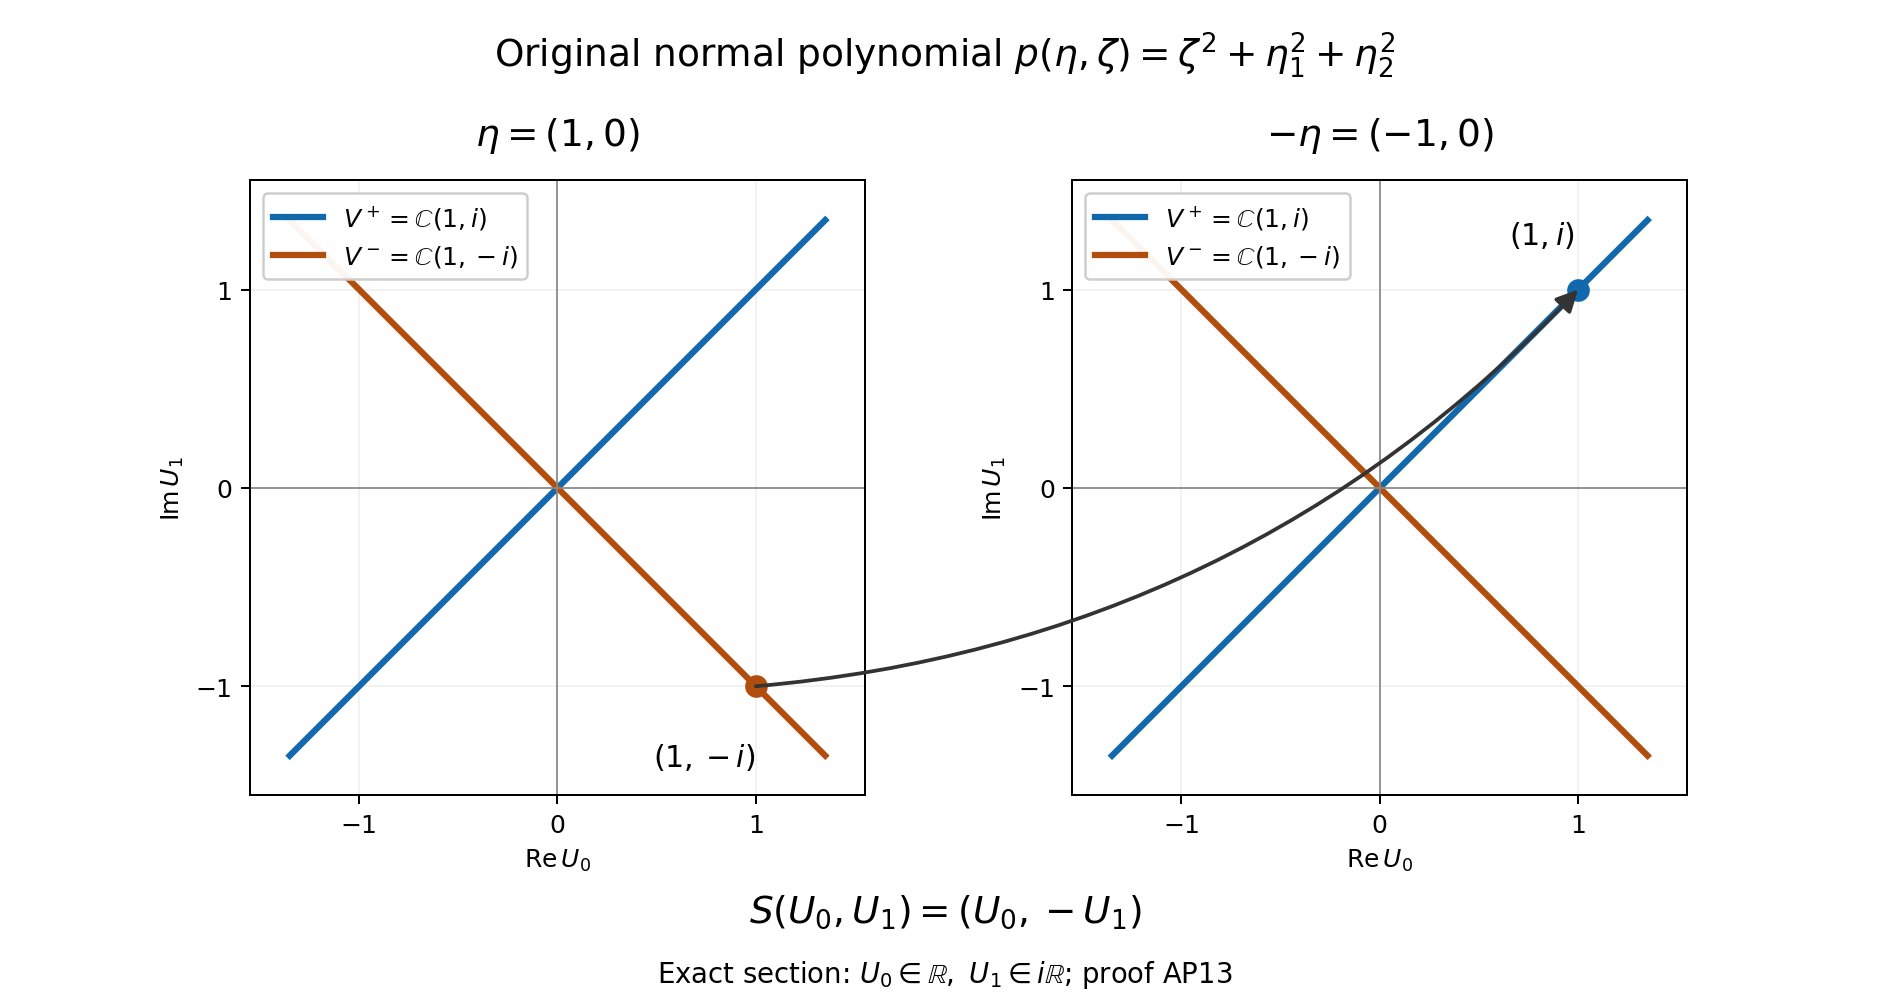
\includegraphics[keepaspectratio,alt={Reflection of original complex Cauchy jets on an exact real section}]{../figures/calderon-antipodal-jets.png}}
\caption{Reflection of original complex Cauchy jets on an exact real
section}
\end{figure}

The figure shows the exact section in AP13 for the original scalar
Laplacian and the two indicated covectors. The arrow identifies the
original point \((1,-i)\) with its reflected point \((1,i)\); it does
not depict a trajectory. The full complex jet spaces and their exact
projection remain given by AP13.

The principal identity is not an identity for every lower-order normal
equation. A concrete full differential polynomial is \[
 \begin{gathered}
 P=D_t^2+D_y^2+D_y+1,\qquad
 r(\eta)=\sqrt{\eta^2+\eta+1},\\
 q_{\rm full}(\eta)=\frac12\begin{pmatrix}1&1/(i r(\eta))\\ i r(\eta)&1\end{pmatrix}.
 \end{gathered}
 \tag{AP14}
\] Here \(\eta^2+\eta+1=(\eta+1/2)^2+3/4>0\), so the full frozen
positive and negative solutions are \(e^{-r(\eta)t}\) and
\(e^{r(\eta)t}\). Their jets prove the displayed full projection
directly, with the original \(D_t\) convention and all lower-order terms
retained. Its principal polynomial is the elliptic \(\zeta^2+\eta^2\),
which satisfies AP6. For the full family,
\(S(I-q_{\rm full}(\eta))S=q_{\rm full}(\eta)\), whereas
\(r(-\eta)^2=\eta^2-\eta+1\ne r(\eta)^2\) when \(\eta\ne0\). Positivity
of both square roots then gives
\(q_{\rm full}(-\eta)\ne S(I-q_{\rm full}(\eta))S\). This is a
counterexample for the exact full frozen normal projection; no
identification with a particular global choice of the
smoothing-corrected Green operator is needed or claimed. AP6 concerns
the original principal weighted projection, and the full \(Q\) retains
the distinct Green and smoothing arguments of Sections7--11.

\subsection{10. Why the full defect has a smooth
kernel}\label{why-the-full-defect-has-a-smooth-kernel}

We now prove the stronger operator assertion \[
Q^2-Q\in\Psi^{-\infty}(Y;E^m,E^m).
\tag{CD27}
\] Vanishing of the leading symbol alone would give only one order of
improvement and is insufficient.

First, \(F_0= r^+R_F\mathcal J\) maps boundary distributions
continuously to \(C^\infty(X;F)\) and has a smooth kernel on
\(X\times Y\). In fact (CD14) differentiates the smooth kernel of
\(R_F\) in its input variable a finite number of times and restricts
that variable to \(Y\). Its output derivatives of every order remain
smooth and bounded on the compact working set.

Second, zero extension of \(KU\), initially for smooth \(U\), has a
continuous distributional extension \[
\mathcal E:\mathcal D'(Y;E^m)\longrightarrow
\mathcal E'(\widehat X;E),\qquad \mathcal E U=e^+KU\quad(U\text{ smooth}).
\tag{CD28}
\] Here and below an output cutoff equal to one near \(X\) makes the
displayed compact-support convention literal. Define this extension by
duality: \[
\langle\mathcal E U,\phi\rangle
=\langle\mathcal JU,T^*e^+(r^+\phi)\rangle.
\tag{CD29}
\] The right side uses boundary derivatives through normal order
\(m-1\). Their values are unambiguous. To check this explicitly, \(T^*\)
has order \(-m\), so it takes the localized \(L^2\) section
\(e^+r^+\phi\) into \(H^m\). After any number of tangential derivatives
the result is still locally \(H^m\): commute such derivatives through
\(T^*\); each commutator is again of order \(-m\), and tangential
differentiation commutes with zero extension. Iterating, with compact
cutoffs, proves the assertion to every tangential order. Fourier
Cauchy--Schwarz in the tangential variables and the one-dimensional
inequality \(H^m(\mathbb R)\subset C^{m-1}(\mathbb R)\) now give common
two-sided values of every required normal derivative. The
one-dimensional inequality follows directly by integrating
\(|\tau|^{m-1}\widehat w(\tau)\) against the \(H^m\) weight, since its
squared reciprocal tail is \(O(|\tau|^{-2})\). In addition, the adjoint
transmission proved in Section 5 gives smooth one-sided restrictions,
continuously in the smooth seminorms of \(\phi\).

It follows that the transpose boundary expression applied to
\(T^*e^+r^+\phi\) is a smooth section of the dual Cauchy bundle,
continuously in \(\phi\). Pairing with any boundary distribution defines
(CD29) and proves its continuity. For smooth \(U\), approximate
\(r^+\phi\) by functions vanishing near \(Y\), using cutoffs depending
only on \(t\). Their zero extensions converge in \(L^2\), with every
tangential derivative. The preceding \(H^m\) argument makes the relevant
boundary derivatives of their images under \(T^*\) converge. Ordinary
distributional duality away from \(Y\) gives (CD29) for each
approximation; passing to the limit gives \(\langle e^+KU,\phi\rangle\),
proving (CD28). No multiplication of an arbitrary distribution by the
discontinuous indicator of \(X\) was used.

The map \(\gamma r^+R_E\mathcal E\) has a smooth kernel on
\(Y\times Y\). This can be proved directly, without interpreting weak
continuity as smoothing: insert each smooth input-variable kernel
section of \(R_E\) into (CD29). It depends smoothly on the output point
with all derivatives; the continuous adjoint-transmission map in (CD29)
makes its resulting boundary section jointly smooth. Differentiating
this section proves the smooth-kernel assertion. Similarly
\(\gamma r^+Te^+F_0\) has a smooth kernel: for each boundary input point
its \(F_0\)-kernel section is smooth on \(X\), smoothly depending on
that point, and the smooth transmission map \(\gamma r^+Te^+\) preserves
this dependence.

Apply (CD19) to \(u=KU\), for smooth \(U\). By (CD16) and (CD17) it
gives \[
QU+\gamma r^+R_E\mathcal E U
=\gamma r^+Te^+F_0U+Q^2U.
\tag{CD30}
\] Thus \(Q^2-Q=\gamma r^+R_E\mathcal E-\gamma r^+Te^+F_0\), a
difference of the two smooth kernels just proved. Smooth boundary
functions are distributionally dense by chartwise convolution and
partition, and every operator in the identity is continuous on
distributions. Therefore the identity and (CD27) hold on all boundary
distributions. The argument proves smoothing at every order, with the
actual remainder kernels from (CD10), and never assumes (CD27) in order
to define \(\mathcal E\).

\subsection{11. The positive trace of an interior particular
solution}\label{the-positive-trace-of-an-interior-particular-solution}

The particular-solution trace obeys the useful gain \[
QV:\bar H^0(X^\circ;F)\longrightarrow C^\infty(Y;E^m)
\quad\text{continuously},\qquad V=\gamma r^+Te^+.
\tag{CD31}
\] The factor here is \(Q\), with the inward convention of (CD12).

For smooth \(f\), let \(u=r^+Te^+f\), smooth by transmission. Then
\(Pu=f+r^+R_Fe^+f\), while \(\gamma u=Vf\). Insert these into (CD19) and
cancel \(\gamma u=Vf\). The exact remaining identity is \[
QVf=\gamma r^+R_Ee^+r^+Te^+f
-\gamma r^+Te^+r^+R_Fe^+f.
\tag{CD32}
\] Each term is continuously smooth for \(f\in L^2\). For the first,
zero extension is bounded in \(L^2\), the local order \(-m\) theorem
gives \(Te^+f\in H^m\), restriction and then zero extension are bounded
in \(L^2\), and \(R_E\) is smoothing. For the second, \(R_F e^+\) is
continuously smooth on a neighborhood of \(X\), so its restriction,
followed by the smooth transmission map of \(T\) and the boundary trace,
is smooth. The bounds apply to every output derivative. Also
\(V:L^2\to\mathcal H_m\) is continuous by the same \(H^m\) estimate and
(CD3), so the left side of (CD32) is already well-defined for \(L^2\)
inputs by (CD21). Smooth approximation in \(L^2\) extends the equality
and proves (CD31). This derivation keeps both parametrix remainders and
does not require an invertible extension.

\subsection{12. What the boundary reduction actually
says}\label{what-the-boundary-reduction-actually-says}

For a smooth solution of \(Pu=f\), set \(U=\gamma u\). With
\(\mathcal B=(\mathcal B_{jk})\) from (CD6), the exact boundary
identities are \[
U=\psi+QU,\qquad \mathcal BU=g,\qquad
\psi=Vf-Su.
\tag{CD33}
\] The term \(Su\) is smoothing in the interior unknown, whereas \(Vf\)
is fixed by the forcing. Thus the first equation determines the
nonpositive-mode component of the Cauchy vector, modulo a smoothing
term. The trace of the forcing has \(QVf\) smooth by Section 11; \(QSu\)
is also smooth, since pseudodifferential operators preserve smooth
sections. In particular \(Q\psi\) is smoothing in \((f,u)\),
quantitatively for \(f,u\in L^2\). This explains the compatibility among
the apparent \(mN\) Cauchy equations: at the symbol level \((I-q)U\) is
prescribed and the remaining data lie in \(\operatorname{ran}q\).

For every \(s\geq m\), (CD33) has the spaces \[
U\in\mathcal H_s,\quad f\in\bar H^{s-m},\quad
g_j\in H^{s-m_j-1/2}(Y;G_j),\quad
\mathcal B:\mathcal H_s\to\bigoplus_jH^{s-m_j-1/2}(Y;G_j).
\tag{CD34}
\] The particular trace \(Vf\) has this regularity when \(f=Pu\) with
\(u\in\bar H^s\), by (CD19): both \(U\) and \(QU\) lie in
\(\mathcal H_s\), and \(Su\) is smooth. Independently \(V\) on arbitrary
\(\bar H^{s-m}\) requires the appropriate truncated-operator mapping
theorem for that scale; it is not deduced from the unrestricted zero
extension \(e^+:\bar H^{s-m}\to H^{s-m}\), which can fail. The exact
\(L^2\) statement needed above has already been proved. The adjoining
boundary Fredholm unit establishes the further mapping and projected
inverse statements.

Conversely, simply choosing \(U\) satisfying a version of (CD33) with
the smoothing term omitted is not an exact existence proof for the
original differential problem. The remainders (CD17)--(CD19) must be
corrected or included in a Fredholm argument. This lesson supplies the
full Cauchy construction and the compatible weighted symbol, and leaves
that general solvability obligation to its separate proof.

\subsection{13. Four calculations that expose different
constraints}\label{four-calculations-that-expose-different-constraints}

\textbf{A first-order system with a changing stable rank.} On a
two-dimensional collar consider \(P=D_tI-iAD_y\), where \(A=2I+N\) on
\(\mathbb C^2\), \(N\ne0\), \(N^2=0\). Its principal determinant is
\((\zeta-2i\eta)^2\), nonzero for every real \((\eta,\zeta)\ne0\). The
normal solution is \[
v(t)=e^{-2\eta t}(I-\eta tN)v(0).
\tag{CD35}
\] For \(\eta>0\) every initial vector is stable, whereas for \(\eta<0\)
no nonzero initial vector is stable. Thus \(q(\eta)=I\) on the positive
ray and \(q(\eta)=0\) on the negative ray. The polynomial factor retains
the generalized modes. At a given boundary point a differential boundary
target bundle has a single fixed rank, so it cannot be bijective from
both a rank-two and a rank-zero stable space. This is a concrete failure
of the local complementing test for every such choice of target rank,
despite interior ellipticity. It does not assert failure of all possible
nonlocal spectral boundary constructions.

\textbf{A fourth-order datum projected onto two decaying rates.} Freeze
\(p(\zeta)=(\zeta^2+\rho^2)(\zeta^2+9\rho^2)\), \(\rho>0\), and
prescribe \(U=(0,0,1,0)\). The positive modes are \(e^{-\rho t}\) and
\(e^{-3\rho t}\). Their projected combination is \[
v^+(t)=\frac{e^{-\rho t}-e^{-3\rho t}}{16\rho^2},\qquad
qU=\left(0,-\frac{i}{8\rho},\frac12,\frac{13i\rho}{8}\right).
\tag{CD36}
\] To verify the coefficients, decompose \(U\) in the four Cauchy
vectors associated with \(e^{\pm\rho t},e^{\pm3\rho t}\). Vanishing of
the first and third normal jets makes the coefficients of the positive
and corresponding negative exponentials equal in the direct-sum
decomposition. The zeroth jet gives opposite coefficients for the two
rates. The second jet then gives \(16\rho^2a=1\). Applying
\(D_t=-i\partial_t\) yields exactly (CD36). The negative contribution in
the direct-sum decomposition is subtracted to obtain the actual \(v^-\)
in (CD25). This computation exhibits the distinct powers \(\rho^{k-2}\)
in one column of the weighted projection.

\textbf{A coefficient jet that survives in the jump.} Put
\(P=(1+t)D_t^2+D_y^2\) near \(t=0\). Formula (CD14) gives \[
\mathcal J(U_0,U_1)=-iU_0D_t\delta+(-iU_1+U_0)\delta.
\tag{CD37}
\] Indeed \((1+t)D_t\delta=D_t\delta+i\delta\), as is verified by
pairing with a test function. Evaluating \(1+t\) at zero before
multiplying \(D_t\delta\) would delete the \(U_0\delta\) term. That term
is lower in the tangential order but indispensable in the exact Green
identity and the full projection defect proof.

\textbf{An idempotent leading symbol is not enough.} On the circle let
\(\Lambda=(1+D_y^2)^{1/2}\), defined by its Fourier multipliers, and let
\(\Pi=\operatorname{diag}(1,0)\). The classical order-zero matrix
\(A=\Pi+\Lambda^{-1}I\) has leading symbol \(\Pi\), but \[
A^2-A=(2\Pi-I)\Lambda^{-1}+\Lambda^{-2}I.
\tag{CD38}
\] Its first diagonal Fourier multiplier is
\(\langle n\rangle^{-1}+\langle n\rangle^{-2}\), which does not decrease
faster than every inverse power. A smooth kernel on the compact circle
would have such rapid Fourier decay by integration by parts in both
variables. Hence (CD38) is not smoothing. This is a generic
pseudodifferential matrix, not the operator built from (CD16); it shows
exactly what the Green identity contributes beyond the residue
calculation.

\subsection{14. Exercises with complete
solutions}\label{exercises-with-complete-solutions}

\textbf{1. Retain noncommuting coefficients.} For constant matrices
\(A,B,C\), with \(A\) invertible, take \(p(\zeta)=A\zeta^2+B\zeta+C\).
Write the jump distribution and the four leading projection entries,
leaving the contour unevaluated.

\textbf{Solution.} The jump is \(-i[AU_0D_t\delta+(AU_1+BU_0)\delta]\).
Formula (CD22) gives the contour integral of the block matrix \[
\begin{pmatrix}
p^{-1}(B+\zeta A)&p^{-1}A\\
\zeta p^{-1}(B+\zeta A)&\zeta p^{-1}A
\end{pmatrix}
\tag{CD39}
\] divided by \(2\pi i\). Each block is an ordered product. In
particular \(p^{-1}B\) cannot in general be replaced by \(Bp^{-1}\):
multiplying their difference on the left and right by \(p\) gives the
commutator \(Bp-pB\), which can be nonzero. For a tangential principal
polynomial \(A\) has degree zero, \(B\) degree one and \(C\) degree two,
so the entries after normal integration have degrees \(0,-1,1,0\),
respectively.

\textbf{2. Check the jet rescaling.} Define
\(D_r=\operatorname{diag}(1,r,\ldots,r^{m-1})\). Show how \(q(y,r\eta)\)
is recovered from \(q(y,\eta)\), and explain why this does not change
its rank.

\textbf{Solution.} The \((k,l)\)-entry of \(D_rq(y,\eta)D_r^{-1}\) is
\(r^{k-l}q_{kl}(y,\eta)\), equal to \(q_{kl}(y,r\eta)\) by (CD22). Thus
the two projections are conjugate by an invertible matrix. Their images
and kernels have the same dimensions. The unweighted Euclidean norm of
their entries can grow with \(r\); that growth is absorbed by the
Sobolev weights in (CD2), rather than contradicting projection rank
invariance.

\textbf{3. Locate the trace threshold.} Explain why the proof of (CD3)
cannot be continued to \(r=k+1/2\), and construct bounded \(H^{k+1/2}\)
functions whose \(k\)-th normal traces grow.

\textbf{Solution.} The reciprocal-weight integral has tail
\(\int_1^R\tau^{-1}d\tau=\log R\). Take a fixed smooth tangential
Fourier factor \(\varphi(\eta)\) supported where \(|\eta|<1\), and set
\(\widehat w_R(\eta,\tau)=\varphi(\eta)(\log R)^{-1/2}\tau^{-k-1}\chi_R(\tau)\),
where \(\chi_R\) is a smooth cutoff supported in \([1,2R]\), equal to
one on \([2,R]\), with uniformly scaled endpoints. The squared
\(H^{k+1/2}\) norm is bounded by a constant times
\((\log R)^{-1}\int_1^{2R}\tau^{-1}d\tau\), hence uniformly bounded. Its
\(k\)-th trace has tangential Fourier transform a constant multiple of
\(\varphi(\eta)\sqrt{\log R}\), up to a bounded relative error tending
to zero. Its \(H^0\) norm therefore grows. Each \(w_R\) is smooth by its
compact smooth Fourier support. This disproves a bounded trace into the
predicted endpoint target; it does not contradict traces on a solution
subspace with additional elliptic information.

\textbf{4. High tangential order is permitted.} For an order-two
elliptic equation take the reduced boundary operator \(B=D_y^7D_t\).
State its target on \(\bar H^2\), and compare it with \(D_t^8\).

\textbf{Solution.} The total order is eight and the normal order is one.
The trace \(\gamma_1u\) is in \(H^{1/2}\), so seven tangential
derivatives give \(Bu\in H^{-13/2}\). This is the target \(H^{2-8-1/2}\)
in (CD7). The expression \(D_t^8u|_Y\) is not an ordinary trace for a
general \(H^2\) section. Normal division uses the equation to replace it
by a reduced operator and a boundary differential expression in the
forcing. The latter expression is meaningful for smooth forcing, but it
is not automatically defined for arbitrary \(L^2\) forcing.

\textbf{5. Separate the two halves of complementing.} For the frozen
polynomial \(\zeta^2+\rho^2\), \(\rho>0\), measure both \(v(0)\) and
\(D_tv(0)\) with target \(\mathbb C^2\). Is the resulting boundary map
complementing?

\textbf{Solution.} Every stable solution is \(v(t)=a e^{-\rho t}\), and
its two measurements are \((a,i\rho a)\). This map is injective, but its
range is the one-dimensional line with second coordinate \(i\rho\) times
the first. It is not surjective onto \(\mathbb C^2\), so it is not
complementing. With only the first measurement and target \(\mathbb C\)
it is bijective. This frozen calculation is a test of principal boundary
data; a global solvability theorem still requires its analytic argument.

\textbf{6. Determine the negative-side sign.} If \(U\) is the Cauchy
vector of a negative stable solution \(w^-\), what are the two functions
obtained from (CD23)?

\textbf{Solution.} Equation (CD26) gives \(qU=0\). Hence
\(\gamma v^+=0\), so ODE uniqueness gives \(v^+=0\). The jump equation
then reads \(-\gamma v^-=U=\gamma w^-\), and uniqueness gives
\(v^-=-w^-\). The minus sign is forced by the convention ``positive
trace minus negative trace'' in (CD25). Replacing it by \(+w^-\) would
reverse the source term in (CD24).

\textbf{7. Perturb the parametrix by a smooth kernel.} Let \(T'=T+L\),
where \(L\) has a properly supported smooth kernel. Show explicitly that
the corresponding \(Q'\) differs from \(Q\) by a smooth kernel, while an
exact identity \(Q'=Q\) need not hold.

\textbf{Solution.} The difference is \(\gamma r^+L\mathcal J\). In a
local expression (CD14), integration against the derivative of
\(\delta\) differentiates the input-variable kernel of \(L\), including
the coefficient factors, and restricts it to \(Y\). Tangential
derivatives from \(P_a\) do the same in the tangential input variables.
The final \(\gamma\) takes finitely many output normal derivatives and
restricts the output to \(Y\). Thus all resulting entries are smooth on
\(Y\times Y\). They need not vanish: choosing a separated kernel
\(L(x,z)=a(x)b(z)^*\) with a nonzero relevant input boundary jet and a
nonzero output boundary jet generally gives a nonzero finite-rank
difference. The principal projection is unchanged, but the full
approximate projection has changed.

\textbf{8. Recover every jump from the top coefficient.} Suppose a
piecewise normal ODE solution has singular forcing equal to (CD24).
Prove that matching only the highest derivative of \(\delta\) and the
invertibility of \(p_m\) starts a complete recovery of all \(m\) jumps.

\textbf{Solution.} At derivative order \(m-1-r\), the coefficient of the
difference between the actual forcing and (CD24), multiplied by \(i\),
is \(p_m(W_r-U_r)+\sum_{l<r}p_{m-r+l}(W_l-U_l)\). For \(r=0\) the sum is
empty, and \(p_m\) invertible gives \(W_0=U_0\). If the equalities hold
for \(l<r\), the sum vanishes and the same invertibility gives
\(W_r=U_r\). Induction reaches \(r=m-1\). No root simplicity is used,
and no inverse is commuted through a coefficient. This triangular
mechanism is the algebraic content behind the full distributional jump.

\subsection{15. The exact receiving boundary
distribution}\label{the-exact-receiving-boundary-distribution}

Every original normal coefficient jet in the boundary distribution \[
\mathcal JU=i^{-1}\sum_{l=0}^{m-1}\sum_{j=0}^{m-1-l}
P_{j+l+1}(t,y,D_y)\big(U_l(y)D_t^j\delta(t)\big).
\tag{CJ19}
\] is unchanged. This is the whole original (CD14), with its triangular
index range, its factor \(i^{-1}\), and coefficients acting after
multiplication by the normal delta derivative. A test supported away
from \(Y\) has every normal derivative zero along \(Y\), so each pairing
in (CJ19) vanishes; the support remains on the compact original
boundary. Coefficient multiplication against a delta derivative uses the
actual normal jets up to that derivative order. Equations (CJ6)--(CJ7)
preserve all of them, so the extension changes no term of this boundary
operator or of the exact jump identity (CD15).

Choose a relatively compact open neighborhood of \(X\) inside the
displayed ambient domain by retaining the negative collar only through
\(-\delta/2\). Its closure lies inside that domain since \(X\) and \(Y\)
are compact. The existing properly supported bundle calculus therefore
applies there to this full original differential extension and supplies
(CD10) with both original error sides. This completes the globalization,
bundle transport, smooth supported coefficient extension and ellipticity
persistence used in Section 4. It asserts neither an invertible closed
double nor an exact solution obtained by dropping a smoothing remainder.

\subsection{Further questions and
references}\label{further-questions-and-references}

Lashi Bandara, Magnus Goffeng and Hemanth Saratchandran,
\href{https://arxiv.org/abs/2104.01919v2}{\emph{Realisations of elliptic
operators on compact manifolds with boundary}, arXiv:2104.01919v2},
Sections 3.1--3.2 and 9, supply a freely accessible higher-order
treatment of the graded jets, approximate and exact Calderón
projections, and the mixed regularity of maximal-domain traces. Their
Section 3.1 states the approximate projection theorem by citation;
Sections 5--11 above give the complete receiving proof with every layer
order and both smoothing remainders.

The separate editorial note
\href{../supplements/calderon-conventions-and-mixed-orders.html}{Calderón
projections: trace phases, residues and boundary norms}, BC1--BC28,
proves the exact change between their ordinary derivative traces and our
original D traces. It corrects the source's printed trace phase, residue
phase and row-versus-column degree using complete scalar counterexamples
and the unchanged original matrix products. It also records the exact
antipodal rank qualification and proves a Fourier model of their
off-diagonal compactness condition. These corrections concern the
identified source version; the construction and mathematical formulas
above are retained. The source's additional global Hardy-space and
sectorial-projector statements require their respective proofs and are
not deduced from an approximate projection alone.

Three next questions distinguish what the construction already gives
from what requires further work. First, a boundary matrix bijective on
\(\operatorname{ran}q\) suggests an inverse on that projected symbol
bundle. Constructing a full operator inverse modulo compact remainders,
with all Sobolev orders and smooth cokernel descriptions, is the next
Fredholm problem. Second, an approximate projection can sometimes be
corrected by a smoothing operator to an exact projection with an
appropriate global Cauchy range. Its finite-dimensional correction and
dependence on the extension must be proved, rather than inferred from
(CD27). Third, parameter-dependent stable bundles can carry topological
obstructions to local differential boundary conditions, as the first
worked model already detects at the rank level. More refined
obstructions require global bundle and index arguments.

\end{document}
